\chapter{Theory}\label{c:Theory}

\section{Standard Model}


The Standard Model (SM) of particle physics is a collection of several theories that provides the most accurate theoretical framework for describing all known components of matter and their interactions to date. The model describes three fundamental forces that control interactions between the constituents, each force mediated by an integer spin particle called a \textit{gauge boson}, and the spin-$\frac{1}{2}$ \textit{quarks} and \textit{leptons} that compose all matter. The framework is comprised of quantum field theories where each particle is an excitation of a corresponding field, and the interactions of the fields govern the particle interactions. The mathematical structure is  based on the symmetry group $SU(3)_c\times SU(2)_L\times U(1)_\gamma$ and is required to be gauge-invariant. The SM does not include gravity as gravitational interactions are significantly weaker than the other fundamental forces, so are neglected in this thesis. \note{wording here? of neglected?}

	\subsection{Fermions}
	
		The full set of spin-$\frac{1}{2}$ \textit{fermions}, described in Tables \ref{t:tab:quark} and \ref{t:tab:lepton}, is the combination of the quark and lepton families, which each have three generations of particle.  For each distinct particle there is also an anti-particle which is identical aside from opposite charge and handedness. Most observable matter is made up of solely the first generation of the  up and down quarks, the electron and the electron neutrino. Both the leptons and the quarks obey Fermi-Dirac statistics, with quarks experiencing all three fundamental forces, charged leptons interacting via the electromagnetic and weak interactions and neutral leptons experiencing only the weak interaction. 
		
		\begin{table}[ht]
			\caption{Spin-$\frac{1}{2}$ fermions: quarks $q$ \cite{pdg}}
			\label{t:tab:quark}
			\medskip
			\centering
			\begin{tabular}{clcl}\toprule
				Generation & Flavour & Charge / $e$ & Mass / GeV \\\midrule
				1    &     Up $u$      &    +2/3   & 0.002\\
	    &     Down $d$    &    -1/3   & 0.005\\
		    	2    &     Charm $c$      &    +2/3   & 1.28\\
		    	&     Strange $s$    &    -1/3   & 0.096\\
				3    &     Top $t$  &   +2/3   & 173.1\\
	    &     Bottom $b$   &   -1/3   & 4.18\\\bottomrule
			\end{tabular}\\[5pt]
		\end{table}
		\begin{table}[ht]
			\caption{Spin-$\frac{1}{2}$ fermions: leptons $l$ \cite{pdg}}
			\label{t:tab:lepton}
			\medskip
			\centering
			\begin{tabular}{clcl}\toprule
				Generation & Flavour & Charge / $e$ & Mass / MeV\\\midrule
				1    &     Electron $e$      &    -1   & 0.511\\
				&     Electron Neutrino $\nu_e$    &   0  & $\sim$0\\
				2    &     Muon $\mu$      &    -1   & 105.658\\
				&     Muon Neutrino $\nu_\mu$    &    0   & $\sim$0\\
				3    &     Tau $\tau$  &   -1   & 1776.86\\
				&     Tau Neutrino $\nu_\tau$   &   0   & $\sim$0\\\bottomrule
			\end{tabular}\\[5pt]
		\end{table}
		\todo{Kinda want these side by side, also debating neutron mass}
		
		Quarks are always confined into colour singlet hadrons bound by the strong interaction, which are either \textit{baryons} ($qqq$) or \textit{mesons} ($q\bar{q}$), like the \textit{proton} ($uud$) and \textit{neutron} ($ddu$). When a high energy hadron is produced, the interaction of the strong force on the quarks results is a collimated \textit{jet} of hadrons that freeze out of the initial hadron. 
		
	\subsection{Forces}
		
		All forces arise due the exchange of unobservable virtual particles, gauge bosons, which obey Bose-Einstein statistics. The three fundamental particle interactive forces for the SM are named the strong, weak and electromagnetic interactions, and are mediated by gluons, weak bosons and photons respectively. The gauge bosons are described in more detail in Table \ref{t:tab:boson}. In addition to the forces, particles acquire mass by coupling to the Higgs field via the spin-0 Higgs boson \cite{gauge-boson-mass, higgs-1, higgs-2}, which is covered in more detail in Section \ref{t:symbreak}. 
		
		\begin{table}[ht]
			\caption{Spin-1 gauge bosons. The strength of the interaction is typical stated in terms of $\alpha$, a dimensionless constant proportional to the matrix element for the virtual particle exchange for each interaction. The weak interaction is intrinsically stronger than the EM interaction, but the mass of the weak bosons limits the range to extremely short distances before the EM interaction is stronger.  The strength of gravity is $\sim 10^{-39}$ hence it is neglected. \cite{pdg}}
			\label{t:tab:boson}
			\medskip
			\centering
			\begin{tabular}{clclc}\toprule
				Interaction & Particle & Charge / $e$ & Mass / GeV & Strength ($\alpha$) \\\midrule
				Strong    &     Gluon $g$      &    0   & 0& $\sim1$\\
				Weak (Charged Current)&     $W^+$    &    1   & 80.4 & \\
				&     $W^-$    &    -1   & 80.4 & $10^{-6}$ \\
				Weak (Neutral Current)&     $Z$   &    0   & 91.2 & \\
				Electromagnetic (EM)   &     Photon $\gamma$  &   0   & 0 & $\frac{1}{137}$\\\bottomrule
			\end{tabular}\\[5pt]
		\end{table}\todo{undecided on the strength column and numbers withinm which were pulled from undergrad notes}
		
		\subsubsection{Quantum Chromodynamics}
		
		Quantum Chromodynamics (QCD) is the theory of the strong interaction, mediated by the gluon which couples to colour charge. It corresponds to the $SU(3)_c$ symmetry group of the overall SM. The strong interaction conserves energy, momentum, angular momentum and colour charge. Only quarks and gluons themselves possess colour charge, so while quarks are the only fermion to feel the strong interaction, gluons can self-couple. This self-coupling of gluons is the reason quarks are always observed in bound states.
		
		\subsubsection{Electroweak Unification} 
		
		Electroweak Unification (EW) is the expression of the electromagnetic interaction described by Quantum Electrodynamics (QED) and the weak interaction as separate manifestations of a combined electroweak force in the Glashow-Weinberg-Salam model \cite{gws-g, gws-w, gws-s}, which corresponds to the $SU(2)_L\times U(1)_\gamma$ symmetry group. QED describes the macroscopically observable $U(1)$ electromagnetic force  with the photon as the mediating boson, and any interactions conserves energy, momentum, parity and charge and additionally never changes particle type through the interaction. The $SU(2)$ weak interaction is mediated by the charged current vector bosons $W^+$, $W^-$ and the neutral current vector boson $Z$, which have large masses that limit the weak interaction to very short distances. The charged current interaction is capable of changing the flavour of a particle and also of violating parity in an interaction. 
		
		The weak interaction by itself was observed to diverge from observation at high energies, leading to the introduction of the unified theory. The combined  $SU(2)_L\times U(1)_\gamma$ group produces four gauge bosons which mix to produce the more recognisable $\gamma$, $W^+$, $W^-$  and $Z$ bosons. The unified force couples to weak isospin, which allows self-coupling between the massive vector bosons, but not the photon as it does not carry electric charge.
		
		While the weak interaction acts on both quarks and leptons, the quark sector is affected by the distinction between the mass eigenstates of quarks; the physically observed flavour sets, and the quark eigenstates of the weak interactions which are superpositions of the mass eigenstates. The effect of this quark mixing in the weak interaction is that different flavour changing interactions have different strengths. The mixing of the mass eigenstates ($q$) into weak eigenstates ($q^\prime$) is described by the Cabbibo-Kobayashi-Makasawa matrix \cite{ckm-c, ckm-km}:
		
		\begin{equation}
		\begin{pmatrix}
		d^\prime \\
		s^\prime\\
		b^\prime \\
		\end{pmatrix}
		 = \begin{pmatrix}
		V_{ud} & V_{us} & V_{ub} \\
		V_{cd} & V_{cs} & V_{cb} \\
		V_{td} & V_{ts} & V_{tb} \\
		\end{pmatrix}
	    \begin{pmatrix}
	    d \\
	    s\\
	    b \\
	    \end{pmatrix}
		\end{equation}
		
		
		
	\subsection{Spontaneous Symmetry Breaking: The Higgs Boson}
	\label{t:symbreak}
	
	The gauge field theories used for the QCD and EW models when unaltered require massless gauge bosons in order to preserve gauge invariance, which follows from the Klein-Gordon equation:
	\begin{equation}
		\frac{\partial^2\psi}{\partial t^2} = (\nabla^2 - m^2)\psi
	\end{equation}\todo{which spacing is prefeable}
	 This is satisfactory for the gluon and photon, but a separate theory is required to provide the mass for the $W^\pm$ and $Z$ bosons. The Higgs Mechanism \todo{cite} proposed introducing a scalar field that interacts with the $W^\pm$ and $Z$ fields. In the Lagrangian formulation this results in a term akin to a mass term ($\propto\psi^2$) which effectively links that mass of the bosons to their coupling with this scalar field. This addition to the Lagrangian is still required to preserve the symmetry of the system and respect the gauge invariance, but is also required to have a non-zero expectation value for the field in the vacuum or ground state of space. The Higgs mechanism introduces the scalar field $\phi$ which has a potential energy $V(\phi)$: 
	 \begin{equation}
		 V(\phi) = a\phi^4 - b\phi^2
	 \end{equation} 
	 
	This results in an equilibrium point ($\phi=0$) that respects the symmetry, but is inherently unstable, with an infinite set of degenerate non-zero minima at $|\phi^2|=\frac{b}{2a}$ where the symmetry is \textit{spontaneously} broken. This field in an analogous fashion to the other quantum fields of the SM can produce particles from excitations which form the physical Higgs Scalar Boson $H$. Confirmation of the Higgs boson as part of the SM was only achieved relatively recently \cite{higgs-atlas, higgs-cms}, where a a spin-0 boson consistent with the SM Higgs was observed. Subsequent measurements made have provided agreement on the new particle as the Higgs boson with a mass of $125.09$ GeV \cite{pdg}. Section \ref{t:higgs} covers in more detail the production and behaviour of the Higgs boson in collider experiments.


\section{Physics of \textit{pp} Collisions}

	Experimental efforts to probe the Standard Model in recent times have focused on high-energy collider experiments, where beams of particle with equal energy are collided head on within detectors.  For proton-proton ($pp$) collisions, matters are complicated as the colliding protons are composite particles, which at high energy consist of the three \textit{valence} quarks $uud$ and a sea of virtual quarks and gluons. Collectively these constituents are referred to as \textit{partons} where each parton carries a fraction of the overall hadron momentum, and the interaction in the $pp$ collision consists of elastic scattering between these partons. At a given energy scale $Q^2$ the probability that a parton $i$ carries a fraction $x_i$ of the overall momentum is described by the \textit{parton distribution function} \todo{decide if i want this italicising} (PDF) $f_i(x, Q^2$). These PDFs cannot be calculated from QCD but can be determined from experimental measurements, and collections of PDFs have been assembled from the leading collider experiments \cite{pdfs}.
	 
	In any particle interaction, the probability a particular reaction occurs is in proportion to the cross section of the reaction. The cross section for a short range, hard parton-parton collision is given by $\hat{\sigma}(Q^2)$, where scattering energy scale $Q^2 = x_1x_2E^2_{cm}$ in the parton-parton centre-of-mass frame where $E_{cm}$ is the energy in the centre-of-mass frame. To compute the cross section $\sigma$ for some hard process $pp\rightarrow X$, all possible combinations of incoming partons must be summed over and the momentum fractions integrated over while accounting for the PDFs:
	\begin{equation}
	\sigma = \sum_{i, j = q, g} \int dx_1dx_2f_i(x_1, Q^2)f_j(x_2, Q^2)\hat{\sigma}(Q^2)
	\end{equation}
	\todo{Think I need more here}
	
	\subsection{Geometry?}\todo{Necessary section?, good title?}
	\label{t:geometry}
	
	The high energy protons used in collisions are automatically relativistic in nature, and as the momenta of the colliding partons are not guaranteed to be equal and opposing there is always an unknown element of longitudinal boosting in $pp$ collisions. As a consequence, use of light-cone coordinates and some definitions of convenient quanties can be of benefit to $pp$ collision analyses \cite{lightcone-all-that}.
	
	Typically the momentum in the transverse plane \pt is used for a particle, and the rapidity $y$ of a particle with non-zero \pt is defined:
	\begin{equation}
	y = \frac{1}{2}\ln\frac{E+p_z}{E- p_z}
	\end{equation}  
	
	This rapidity $y$ transforms additively to boosts along the $z$ axis, so any rapidity difference between two objects is invariant to such boosts. For cases where the mass of a particle is negligible (highly relativistic particles) the rapidity can be related to the polar angle of the particle as the pseudo-rapidity $\eta$:
	\begin{equation}
	\eta = -\ln\tan\frac{\theta}{2}
	\end{equation}

\section{Theoretical Predictions}

	\todo{Not sure if this is a good title, or if aspects and commetary on the jet reconstrucion should go here too.}

	\subsection{Monte-Carlo Event Generators}
	
		Use of Monte-Carlo event generators is critical to current high energy physics, where simulations of particle collisions are used to predict and prepare for real data-taking experiments, to obtain datasets of particular particle interactions and to train and optimise the tools used in analyses. Event generation for $pp$ collisions is broken up into a few main steps to reduce the complexity of generating events with $\mathcal{O}(1000)$ final state particles \cite{monte-carlo}:
		
			\begin{itemize}
				\item Hard process: a particular hard scatter event, the heart of the desired process,  is simulated using the PDFS of the incoming components and perturbation theory to the desired accuracy (LO, NLO,. etc.) to evaluate the outgoing partons.
				\item Parton shower: The outgoing shower of partons is evaluated as a step-by-step simulation in momentum scales using QED and QCD, particularly the recursive radiation of gluons, developing an extended shower filled with mostly soft gluons up to a point where perturbation theory is no longer applicable. 
				\item Hadronization: As perurbation theory breaks down, models that account for the confinement of partons into hadrons and converts the coloured partons of the shower step into colourless hadrons.
				\item Underlying event: Accounts for secondary parton interactions between remnants of the proton from the initial hard scatter to produce soft hadrons that overlap with the simulation of the hard process.
				\item Unstable particle decays: Account for the fact produced hadrons may be resonances not stable particles which go on to decay.	
			\end{itemize}
			\todo{Is a list suitable here?}
			
		Most leading generators like \textsc{Pythia} or \textsc{Herwig} make use of this chain of generation, and modern analyses will make use of multiple generators interfaced together to compute different steps with additional accuracy.

\section{The Higgs Boson}
\label{t:higgs}

	Detecting the Standard Model Higgs boson is strongly dependent of the predominant production and decay channels for the Higgs boson, which in turn depend on the specifications(?) of the collider used for the search. In this section the relevant production and decay channels at the Large Hadron Collider (LHC) will be discussed.

	\subsection{Higgs Production}
	
		While there are many various methods for production of a Higgs boson, at the LHC the cross section is dominated by gloun-gloun fusion (ggF) as shown in figure \ref{fig:higgsproductionCS}, with the second largest cross-section arising from vector boson fusion (VBF). Other significant production processes are the WH/ZH or Higgs-strahlung production modes and associated production with top quarks (ttH) \cite{LHCHiggsCS}. 
		
			\begin{figure}[h]
				\centering
				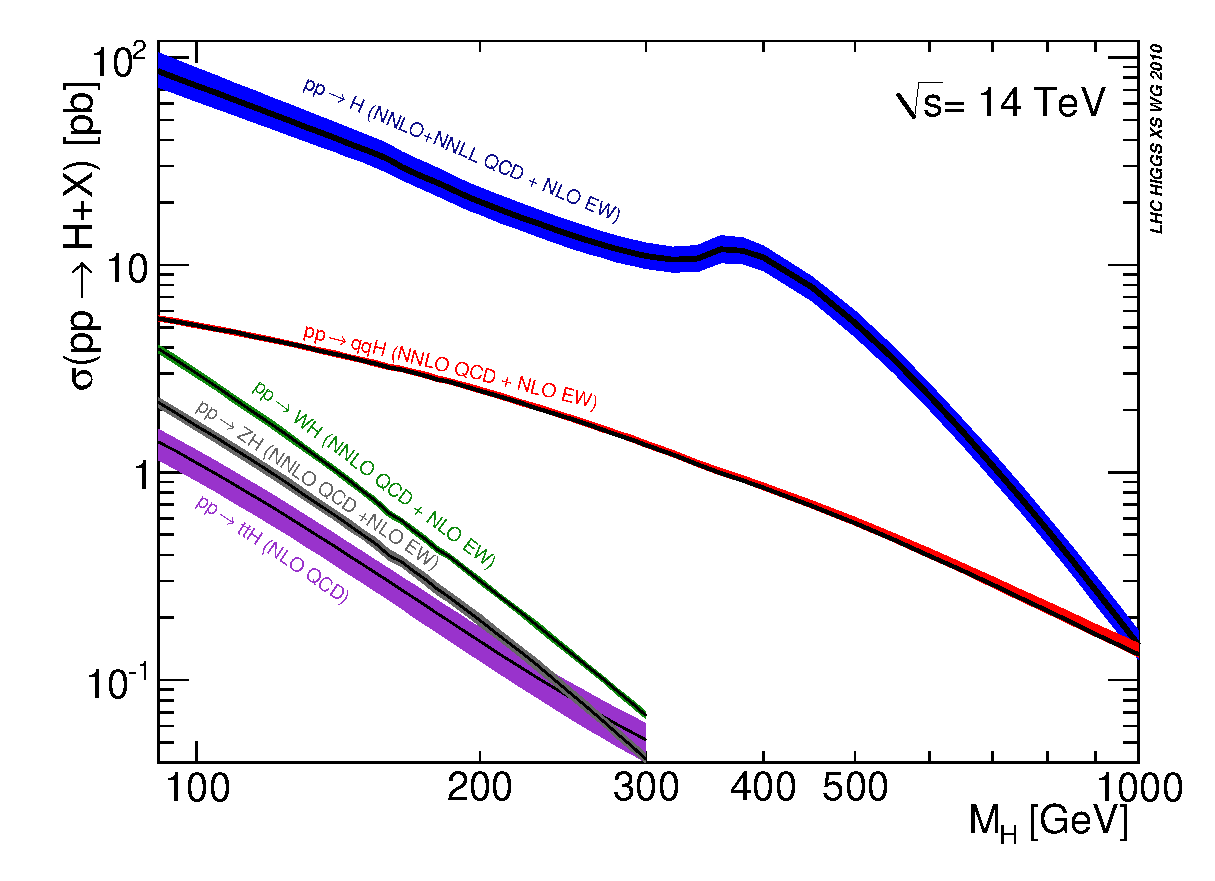
\includegraphics[width=0.7\linewidth]{T/FIGS/YRHXS_Summary_fig3}
				\caption{SM Higgs Production cross section for $\sqrt{s}=14$ TeV. $pp\rightarrow H$ corresponds to ggF production and $pp\rightarrow qqH$ VBF. \cite{LHCHiggsCS}}
				\label{fig:higgsproductionCS}
			\end{figure}
		
		\subsubsection{Gluon-gluon fusion}5555
		
		The dominant production mechanism for the Higgs boson in hadron colliders is the \ggF production via in intermediate quark loop. The dynamics of this mechanism are controlled by strong interactions, thus calculations of QCD corrections are necessary for any accurate predictions, and have been computed up from next-to-leading order (NLO) to N$^3$LO for the ggF process in recent years, along with the inclusion of Electro-Weak corrections in the cross section calculations \cite{LHCHiggsCS}. 
		
			\begin{figure}[h]
			\centering
			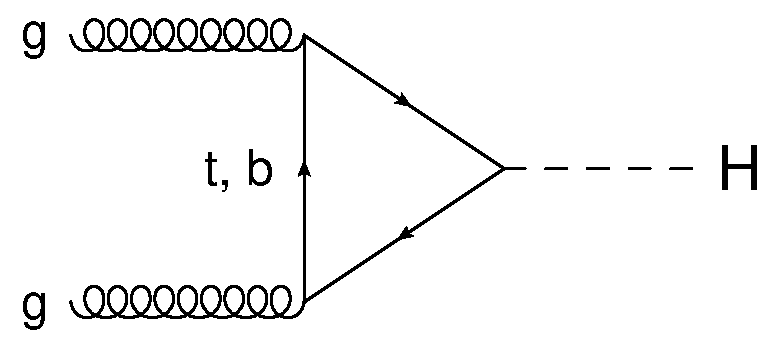
\includegraphics[width=0.4\linewidth]{T/FIGS/ggF}
			\caption{Lowest order Feynmann diagram contributing to \ggF.}
			\label{fig:ggf}
			\end{figure}
			
		\subsubsection{Vector Boson Fusion}
		
			Production of a Higgs boson from the fusion of vector bosons radiated from initial-state quarks is the second largest cross-section at the LHC, as is useful as a production mode due to topological characteristics which can distinguish the event from \ggF. In \VBFHBB, the characteristic topology is a pair central \bjets forming the higgs candidate, and two forward VBF jets formed of remnants of the initially colliding protons as displayed in Figure \ref{fig:T:vbf}. In addition central jet activity is suppressed due to the lack of colour exchange between quarks \cite{VBF2004}.  These distinct features mean that while the cross section for VBF at a Higgs mass of $< 200$ GeV is dominated by ggF, the easy to detect signature means the channel is a cornerstone of searches for the Higgs boson.
		
			\begin{figure}[h]
				\centering
				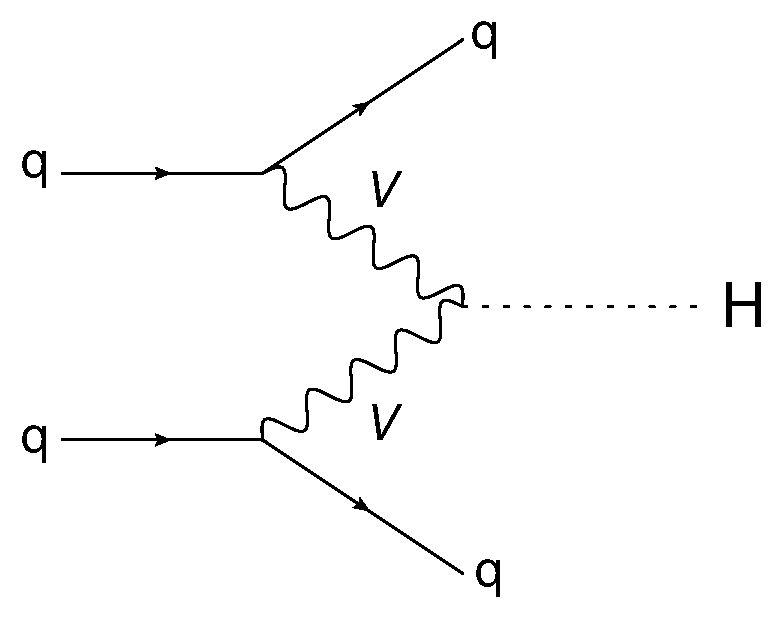
\includegraphics[width=0.4\linewidth]{T/FIGS/vbf}
				\caption{Feynmann diagram for the production of a Higgs boson via vector boson ($V$) fusion, where q denotes any quark or antiquark}
				\label{fig:T:vbf}
			\end{figure}
				
	\subsection{Higgs Decay} 
	
		The branching ratios for decays of the Higgs boson in the Standard Model have been extensively determined using Monte-Carlo event generators. As is to be expected, the relative cross-sections of the decay modes are strongly dependent on the mass of the Higgs boson, as highlighted in Figure \ref{fig:higgsbrlm}. 
	
		\begin{figure}[h]
			\centering
			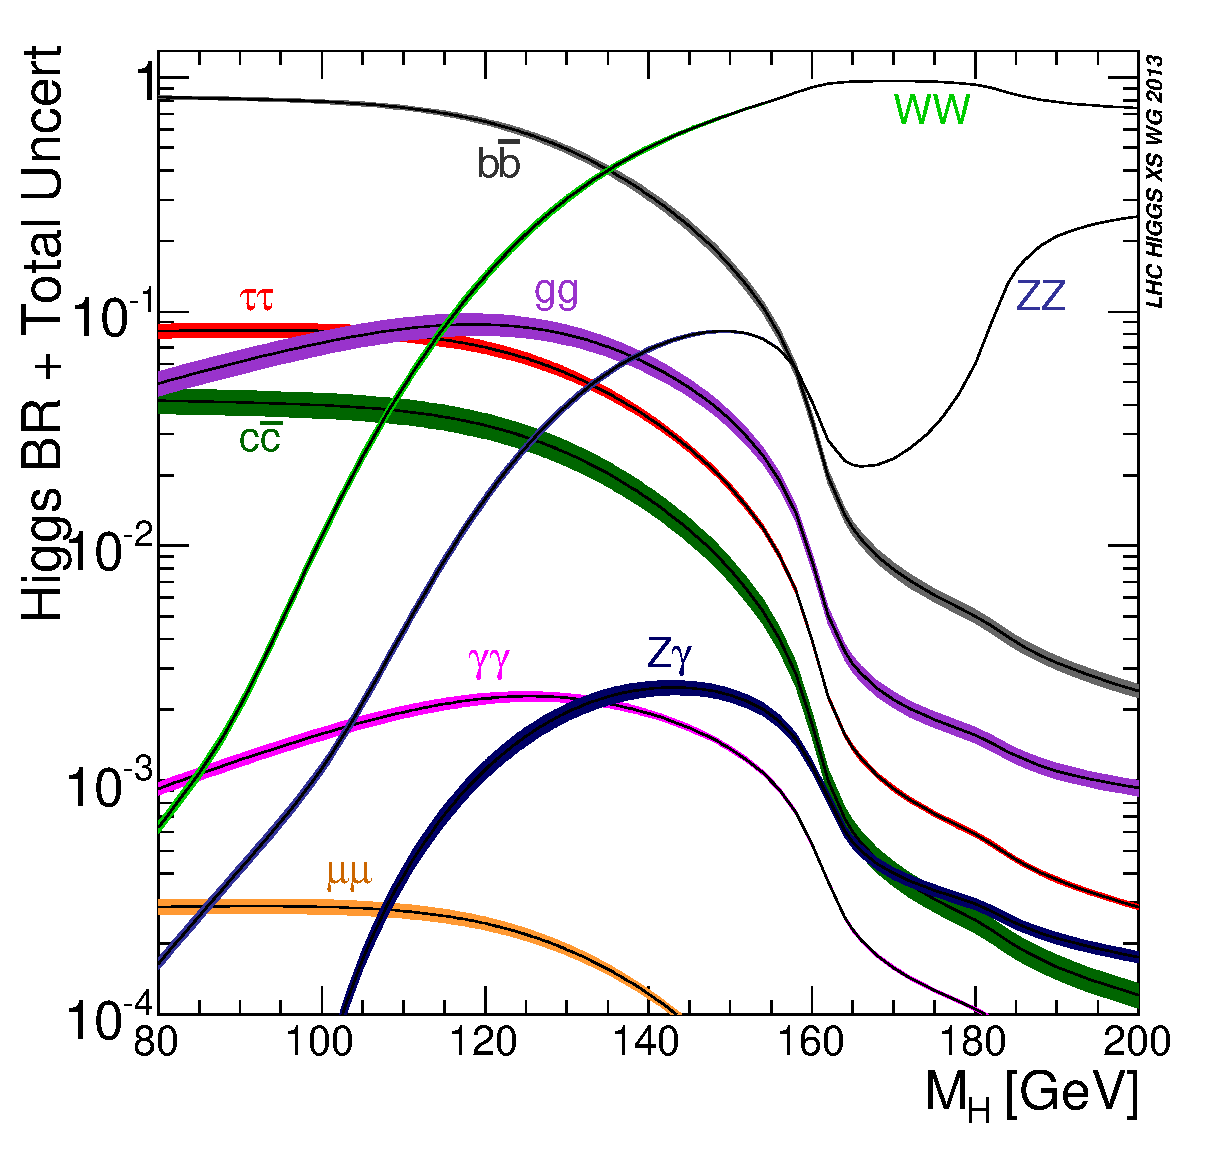
\includegraphics[width=0.5\linewidth]{T/FIGS/Higgs_BR_LM}
			\caption{Higgs decay branching ratios for the low mass region with their uncertainties \cite{LHCHiggsXS2013}.}
			\label{fig:higgsbrlm}
		\end{figure}
		
		While observations consistent with the Standard Model Higgs boson have been made for the $H\rightarrow \gamma\gamma$, $H\rightarrow ZZ$, $H\rightarrow W^+W^-$ and $H\rightarrow \tau^+\tau^-$ channels, observation of th $H\rightarrow bb$ decay channel is significantly hindered owing to the large background from multijet production (Section \ref{T:multijer} maybe?) in hadron collisions. Despite this, the topology of the VBF production mechanism makes it a viable option for observation of the  $b\bar{b}$ decay channel.

	
	\subsection{Vector Boson Fusion}
	
	
	
	
\endinput
